% Options for packages loaded elsewhere
\PassOptionsToPackage{unicode}{hyperref}
\PassOptionsToPackage{hyphens}{url}
%
\documentclass[
]{article}
\title{Occupancy-lab}
\author{Nick Gulotta}
\date{10/27/2021}

\usepackage{amsmath,amssymb}
\usepackage{lmodern}
\usepackage{iftex}
\ifPDFTeX
  \usepackage[T1]{fontenc}
  \usepackage[utf8]{inputenc}
  \usepackage{textcomp} % provide euro and other symbols
\else % if luatex or xetex
  \usepackage{unicode-math}
  \defaultfontfeatures{Scale=MatchLowercase}
  \defaultfontfeatures[\rmfamily]{Ligatures=TeX,Scale=1}
\fi
% Use upquote if available, for straight quotes in verbatim environments
\IfFileExists{upquote.sty}{\usepackage{upquote}}{}
\IfFileExists{microtype.sty}{% use microtype if available
  \usepackage[]{microtype}
  \UseMicrotypeSet[protrusion]{basicmath} % disable protrusion for tt fonts
}{}
\makeatletter
\@ifundefined{KOMAClassName}{% if non-KOMA class
  \IfFileExists{parskip.sty}{%
    \usepackage{parskip}
  }{% else
    \setlength{\parindent}{0pt}
    \setlength{\parskip}{6pt plus 2pt minus 1pt}}
}{% if KOMA class
  \KOMAoptions{parskip=half}}
\makeatother
\usepackage{xcolor}
\IfFileExists{xurl.sty}{\usepackage{xurl}}{} % add URL line breaks if available
\IfFileExists{bookmark.sty}{\usepackage{bookmark}}{\usepackage{hyperref}}
\hypersetup{
  pdftitle={Occupancy-lab},
  pdfauthor={Nick Gulotta},
  hidelinks,
  pdfcreator={LaTeX via pandoc}}
\urlstyle{same} % disable monospaced font for URLs
\usepackage[margin=1in]{geometry}
\usepackage{color}
\usepackage{fancyvrb}
\newcommand{\VerbBar}{|}
\newcommand{\VERB}{\Verb[commandchars=\\\{\}]}
\DefineVerbatimEnvironment{Highlighting}{Verbatim}{commandchars=\\\{\}}
% Add ',fontsize=\small' for more characters per line
\usepackage{framed}
\definecolor{shadecolor}{RGB}{248,248,248}
\newenvironment{Shaded}{\begin{snugshade}}{\end{snugshade}}
\newcommand{\AlertTok}[1]{\textcolor[rgb]{0.94,0.16,0.16}{#1}}
\newcommand{\AnnotationTok}[1]{\textcolor[rgb]{0.56,0.35,0.01}{\textbf{\textit{#1}}}}
\newcommand{\AttributeTok}[1]{\textcolor[rgb]{0.77,0.63,0.00}{#1}}
\newcommand{\BaseNTok}[1]{\textcolor[rgb]{0.00,0.00,0.81}{#1}}
\newcommand{\BuiltInTok}[1]{#1}
\newcommand{\CharTok}[1]{\textcolor[rgb]{0.31,0.60,0.02}{#1}}
\newcommand{\CommentTok}[1]{\textcolor[rgb]{0.56,0.35,0.01}{\textit{#1}}}
\newcommand{\CommentVarTok}[1]{\textcolor[rgb]{0.56,0.35,0.01}{\textbf{\textit{#1}}}}
\newcommand{\ConstantTok}[1]{\textcolor[rgb]{0.00,0.00,0.00}{#1}}
\newcommand{\ControlFlowTok}[1]{\textcolor[rgb]{0.13,0.29,0.53}{\textbf{#1}}}
\newcommand{\DataTypeTok}[1]{\textcolor[rgb]{0.13,0.29,0.53}{#1}}
\newcommand{\DecValTok}[1]{\textcolor[rgb]{0.00,0.00,0.81}{#1}}
\newcommand{\DocumentationTok}[1]{\textcolor[rgb]{0.56,0.35,0.01}{\textbf{\textit{#1}}}}
\newcommand{\ErrorTok}[1]{\textcolor[rgb]{0.64,0.00,0.00}{\textbf{#1}}}
\newcommand{\ExtensionTok}[1]{#1}
\newcommand{\FloatTok}[1]{\textcolor[rgb]{0.00,0.00,0.81}{#1}}
\newcommand{\FunctionTok}[1]{\textcolor[rgb]{0.00,0.00,0.00}{#1}}
\newcommand{\ImportTok}[1]{#1}
\newcommand{\InformationTok}[1]{\textcolor[rgb]{0.56,0.35,0.01}{\textbf{\textit{#1}}}}
\newcommand{\KeywordTok}[1]{\textcolor[rgb]{0.13,0.29,0.53}{\textbf{#1}}}
\newcommand{\NormalTok}[1]{#1}
\newcommand{\OperatorTok}[1]{\textcolor[rgb]{0.81,0.36,0.00}{\textbf{#1}}}
\newcommand{\OtherTok}[1]{\textcolor[rgb]{0.56,0.35,0.01}{#1}}
\newcommand{\PreprocessorTok}[1]{\textcolor[rgb]{0.56,0.35,0.01}{\textit{#1}}}
\newcommand{\RegionMarkerTok}[1]{#1}
\newcommand{\SpecialCharTok}[1]{\textcolor[rgb]{0.00,0.00,0.00}{#1}}
\newcommand{\SpecialStringTok}[1]{\textcolor[rgb]{0.31,0.60,0.02}{#1}}
\newcommand{\StringTok}[1]{\textcolor[rgb]{0.31,0.60,0.02}{#1}}
\newcommand{\VariableTok}[1]{\textcolor[rgb]{0.00,0.00,0.00}{#1}}
\newcommand{\VerbatimStringTok}[1]{\textcolor[rgb]{0.31,0.60,0.02}{#1}}
\newcommand{\WarningTok}[1]{\textcolor[rgb]{0.56,0.35,0.01}{\textbf{\textit{#1}}}}
\usepackage{graphicx}
\makeatletter
\def\maxwidth{\ifdim\Gin@nat@width>\linewidth\linewidth\else\Gin@nat@width\fi}
\def\maxheight{\ifdim\Gin@nat@height>\textheight\textheight\else\Gin@nat@height\fi}
\makeatother
% Scale images if necessary, so that they will not overflow the page
% margins by default, and it is still possible to overwrite the defaults
% using explicit options in \includegraphics[width, height, ...]{}
\setkeys{Gin}{width=\maxwidth,height=\maxheight,keepaspectratio}
% Set default figure placement to htbp
\makeatletter
\def\fps@figure{htbp}
\makeatother
\setlength{\emergencystretch}{3em} % prevent overfull lines
\providecommand{\tightlist}{%
  \setlength{\itemsep}{0pt}\setlength{\parskip}{0pt}}
\setcounter{secnumdepth}{-\maxdimen} % remove section numbering
\usepackage{booktabs}
\usepackage{longtable}
\usepackage{array}
\usepackage{multirow}
\usepackage{wrapfig}
\usepackage{float}
\usepackage{colortbl}
\usepackage{pdflscape}
\usepackage{tabu}
\usepackage{threeparttable}
\usepackage{threeparttablex}
\usepackage[normalem]{ulem}
\usepackage{makecell}
\usepackage{xcolor}
\ifLuaTeX
  \usepackage{selnolig}  % disable illegal ligatures
\fi

\begin{document}
\maketitle

\hypertarget{null-model}{%
\subsubsection{\texorpdfstring{\textbf{Null
Model}}{Null Model}}\label{null-model}}

\hypertarget{ex.1-null-model-output}{%
\paragraph{\texorpdfstring{\textbf{Ex.1-Null model
output}}{Ex.1-Null model output}}\label{ex.1-null-model-output}}

\begin{Shaded}
\begin{Highlighting}[]
\CommentTok{\#null model}
\NormalTok{nullModel }\OtherTok{\textless{}{-}} \FunctionTok{occu}\NormalTok{(}\SpecialCharTok{\textasciitilde{}}\DecValTok{1} \SpecialCharTok{\textasciitilde{}}\DecValTok{1}\NormalTok{, umf)}
\FunctionTok{summary}\NormalTok{(nullModel)}
\end{Highlighting}
\end{Shaded}

\begin{verbatim}
## 
## Call:
## occu(formula = ~1 ~ 1, data = umf)
## 
## Occupancy (logit-scale):
##  Estimate    SE    z P(>|z|)
##     0.498 0.328 1.52   0.129
## 
## Detection (logit-scale):
##  Estimate    SE      z P(>|z|)
##   -0.0384 0.211 -0.182   0.856
## 
## AIC: 229.0629 
## Number of sites: 50
## optim convergence code: 0
## optim iterations: 13 
## Bootstrap iterations: 0
\end{verbatim}

\begin{Shaded}
\begin{Highlighting}[]
\DocumentationTok{\#\# Occupancy estimate {-} Pr(site is occupied)}
\FunctionTok{backTransform}\NormalTok{(nullModel, }\AttributeTok{type=}\StringTok{"state"}\NormalTok{)}
\end{Highlighting}
\end{Shaded}

\begin{verbatim}
## Backtransformed linear combination(s) of Occupancy estimate(s)
## 
##  Estimate     SE LinComb (Intercept)
##     0.622 0.0771   0.498           1
## 
## Transformation: logistic
\end{verbatim}

\begin{Shaded}
\begin{Highlighting}[]
\DocumentationTok{\#\# Detection estimate {-} Pr(detection | site is occupied)}
\FunctionTok{backTransform}\NormalTok{(nullModel, }\AttributeTok{type=}\StringTok{"det"}\NormalTok{)}
\end{Highlighting}
\end{Shaded}

\begin{verbatim}
## Backtransformed linear combination(s) of Detection estimate(s)
## 
##  Estimate     SE LinComb (Intercept)
##      0.49 0.0528 -0.0384           1
## 
## Transformation: logistic
\end{verbatim}

\hypertarget{ex.1-null-model-interpretation}{%
\paragraph{\texorpdfstring{\textbf{Ex.1-null model
interpretation}}{Ex.1-null model interpretation}}\label{ex.1-null-model-interpretation}}

\begin{itemize}
\item
  The probability that a site is occupied is Ψ = 0.62 (SE= 0.07), and
  the probability of detection on a single visit if the site is occupied
  is p = 0.48 (SE=0.05).
\item
  There is a 0.62 probability that a site will be occupied by a quail,
  and if a quail occupies a given site if you visit that site you have a
  0.48 probability of detecting a quail.
\end{itemize}

\hypertarget{ex.1-vegetation-added-as-covariate}{%
\paragraph{\texorpdfstring{\textbf{Ex.1-Vegetation added as
covariate}}{Ex.1-Vegetation added as covariate}}\label{ex.1-vegetation-added-as-covariate}}

\begin{Shaded}
\begin{Highlighting}[]
\CommentTok{\#model 2 habitat index}
\NormalTok{detNullOccHab }\OtherTok{\textless{}{-}} \FunctionTok{occu}\NormalTok{(}\SpecialCharTok{\textasciitilde{}}\DecValTok{1} \SpecialCharTok{\textasciitilde{}}\NormalTok{veght, umf)}
\FunctionTok{summary}\NormalTok{(detNullOccHab)}
\end{Highlighting}
\end{Shaded}

\begin{verbatim}
## 
## Call:
## occu(formula = ~1 ~ veght, data = umf)
## 
## Occupancy (logit-scale):
##             Estimate    SE     z P(>|z|)
## (Intercept)   -2.012 0.963 -2.09  0.0367
## veght          0.865 0.337  2.57  0.0102
## 
## Detection (logit-scale):
##  Estimate    SE      z P(>|z|)
##   -0.0319 0.209 -0.153   0.879
## 
## AIC: 222.5917 
## Number of sites: 50
## optim convergence code: 0
## optim iterations: 16 
## Bootstrap iterations: 0
\end{verbatim}

\begin{Shaded}
\begin{Highlighting}[]
\CommentTok{\#visualize}
\NormalTok{predData }\OtherTok{\textless{}{-}} \FunctionTok{data.frame}\NormalTok{(}\AttributeTok{veght=}\FunctionTok{seq}\NormalTok{(}\AttributeTok{from=}\DecValTok{1}\NormalTok{, }\AttributeTok{to=}\DecValTok{5}\NormalTok{, }\AttributeTok{length.out=}\DecValTok{10}\NormalTok{))}

\NormalTok{predOcc }\OtherTok{\textless{}{-}} \FunctionTok{predict}\NormalTok{(detNullOccHab, }\AttributeTok{newdata=}\NormalTok{predData,}
                   \AttributeTok{type=}\StringTok{"state"}\NormalTok{, }\AttributeTok{append=}\ConstantTok{TRUE}\NormalTok{)}
\end{Highlighting}
\end{Shaded}

\hypertarget{ex.1--question-c}{%
\paragraph{\texorpdfstring{\textbf{Ex.1- Question c
}}{Ex.1- Question c }}\label{ex.1--question-c}}

\begin{itemize}
\tightlist
\item
  The second model that contains the covariate of vegetation height had
  a lower AIC value. This indicates this model explains more of the
  variation and is essentailly a better model than the null-model.
\end{itemize}

\hypertarget{ex.1-plot}{%
\paragraph{\texorpdfstring{\textbf{EX.1-Plot}}{EX.1-Plot}}\label{ex.1-plot}}

\begin{Shaded}
\begin{Highlighting}[]
\CommentTok{\#plot}
\FunctionTok{plot}\NormalTok{(Predicted }\SpecialCharTok{\textasciitilde{}}\NormalTok{ veght, }\AttributeTok{data=}\NormalTok{predOcc, }\AttributeTok{type=}\StringTok{"l"}\NormalTok{, }\AttributeTok{ylim=}\FunctionTok{c}\NormalTok{(}\DecValTok{0}\NormalTok{,}\DecValTok{1}\NormalTok{),}
     \AttributeTok{xlab=}\StringTok{"Habitat index"}\NormalTok{, }\AttributeTok{ylab=}\StringTok{"Occupancy"}\NormalTok{)}
\FunctionTok{lines}\NormalTok{(lower }\SpecialCharTok{\textasciitilde{}}\NormalTok{ veght, }\AttributeTok{data=}\NormalTok{predOcc, }\AttributeTok{lty=}\DecValTok{2}\NormalTok{)}
\FunctionTok{lines}\NormalTok{(upper }\SpecialCharTok{\textasciitilde{}}\NormalTok{ veght, }\AttributeTok{data=}\NormalTok{predOcc, }\AttributeTok{lty=}\DecValTok{2}\NormalTok{)}
\end{Highlighting}
\end{Shaded}

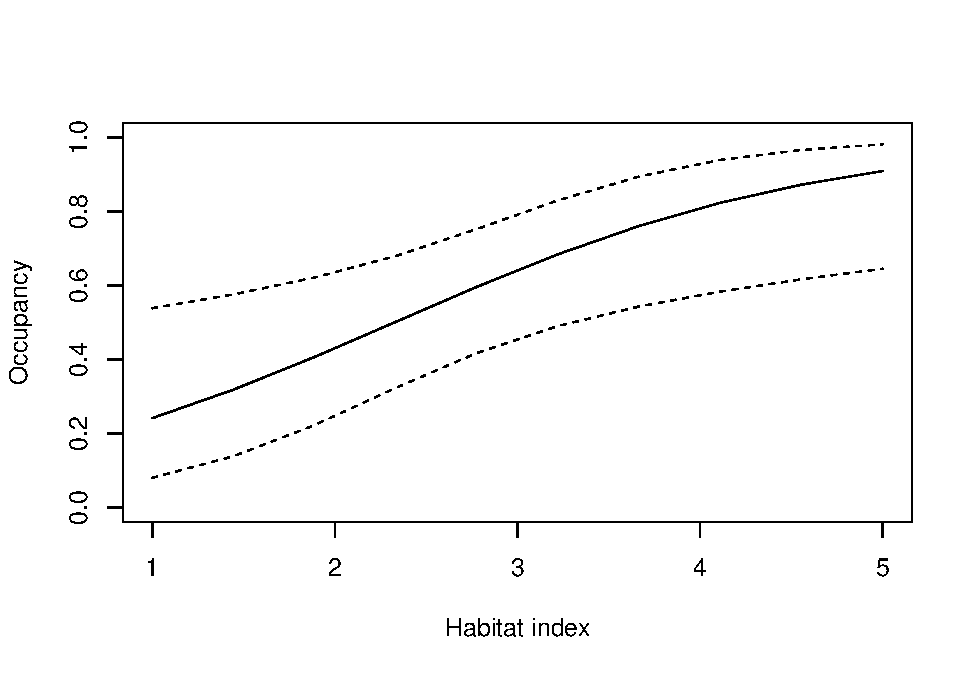
\includegraphics{occupancy-lab_files/figure-latex/plot-1.pdf}

\hypertarget{ex.1-question-d}{%
\paragraph{\texorpdfstring{\textbf{Ex.1-Question
D}}{Ex.1-Question D}}\label{ex.1-question-d}}

\begin{itemize}
\tightlist
\item
  The occurrence probability increases with increasing vegetation
  height. The higher the vegetation the higher probability of quail
  occupying a site.
\end{itemize}

\hypertarget{ex.2-null-model}{%
\paragraph{\texorpdfstring{\textbf{Ex.2-null model
}}{Ex.2-null model }}\label{ex.2-null-model}}

\begin{Shaded}
\begin{Highlighting}[]
\CommentTok{\#null model}
\NormalTok{nullModelMS }\OtherTok{\textless{}{-}} \FunctionTok{colext}\NormalTok{(}\SpecialCharTok{\textasciitilde{}}\DecValTok{1}\NormalTok{, }\SpecialCharTok{\textasciitilde{}}\DecValTok{1}\NormalTok{, }\SpecialCharTok{\textasciitilde{}}\DecValTok{1}\NormalTok{, }\SpecialCharTok{\textasciitilde{}}\DecValTok{1}\NormalTok{, umfMS)}
\FunctionTok{summary}\NormalTok{(nullModelMS)}
\end{Highlighting}
\end{Shaded}

\begin{verbatim}
## 
## Call:
## colext(psiformula = ~1, gammaformula = ~1, epsilonformula = ~1, 
##     pformula = ~1, data = umfMS)
## 
## Initial (logit-scale):
##  Estimate   SE     z P(>|z|)
##      3.88 8.25 0.471   0.638
## 
## Colonization (logit-scale):
##  Estimate   SE     z P(>|z|)
##      4.57 26.8 0.171   0.865
## 
## Extinction (logit-scale):
##  Estimate   SE      z P(>|z|)
##     -8.88 36.7 -0.242   0.809
## 
## Detection (logit-scale):
##  Estimate  SE     z  P(>|z|)
##    -0.877 0.2 -4.39 1.16e-05
## 
## AIC: 173.4767 
## Number of sites: 15
## optim convergence code: 0
## optim iterations: 44 
## Bootstrap iterations: 0
\end{verbatim}

\begin{Shaded}
\begin{Highlighting}[]
\CommentTok{\#backtransform}
\FunctionTok{backTransform}\NormalTok{(nullModelMS, }\AttributeTok{type=}\StringTok{"psi"}\NormalTok{)}
\end{Highlighting}
\end{Shaded}

\begin{verbatim}
## Backtransformed linear combination(s) of Initial estimate(s)
## 
##  Estimate    SE LinComb (Intercept)
##      0.98 0.164    3.88           1
## 
## Transformation: logistic
\end{verbatim}

\begin{Shaded}
\begin{Highlighting}[]
\FunctionTok{backTransform}\NormalTok{(nullModelMS, }\AttributeTok{type=}\StringTok{"col"}\NormalTok{)}
\end{Highlighting}
\end{Shaded}

\begin{verbatim}
## Backtransformed linear combination(s) of Colonization estimate(s)
## 
##  Estimate    SE LinComb (Intercept)
##      0.99 0.272    4.57           1
## 
## Transformation: logistic
\end{verbatim}

\begin{Shaded}
\begin{Highlighting}[]
\FunctionTok{backTransform}\NormalTok{(nullModelMS, }\AttributeTok{type=}\StringTok{"ext"}\NormalTok{)}
\end{Highlighting}
\end{Shaded}

\begin{verbatim}
## Backtransformed linear combination(s) of Extinction estimate(s)
## 
##  Estimate      SE LinComb (Intercept)
##  0.000139 0.00508   -8.88           1
## 
## Transformation: logistic
\end{verbatim}

\begin{Shaded}
\begin{Highlighting}[]
\FunctionTok{backTransform}\NormalTok{(nullModelMS, }\AttributeTok{type=}\StringTok{"det"}\NormalTok{)}
\end{Highlighting}
\end{Shaded}

\begin{verbatim}
## Backtransformed linear combination(s) of Detection estimate(s)
## 
##  Estimate     SE LinComb (Intercept)
##     0.294 0.0415  -0.877           1
## 
## Transformation: logistic
\end{verbatim}

\begin{Shaded}
\begin{Highlighting}[]
\CommentTok{\# create HTML table using kableExtra}
\FunctionTok{library}\NormalTok{(kableExtra)}
\CommentTok{\# create HTML table using kableExtra}
\FunctionTok{library}\NormalTok{(kableExtra)}
\FunctionTok{require}\NormalTok{(knitr)}

\NormalTok{Estimate}\OtherTok{\textless{}{-}}\NormalTok{(}\FunctionTok{c}\NormalTok{(}\FloatTok{0.98}\NormalTok{, }\FloatTok{0.000139}\NormalTok{, }\FloatTok{0.294}\NormalTok{))}
\NormalTok{SE}\OtherTok{\textless{}{-}}\NormalTok{(}\FunctionTok{c}\NormalTok{(}\FloatTok{0.164}\NormalTok{, }\FloatTok{0.00508}\NormalTok{, }\FloatTok{0.0415}\NormalTok{))}
\NormalTok{Term}\OtherTok{\textless{}{-}}\NormalTok{(}\FunctionTok{c}\NormalTok{(}\StringTok{"psi"}\NormalTok{, }\StringTok{"gamma"}\NormalTok{, }\StringTok{"epsilon"}\NormalTok{))}
\NormalTok{tab}\OtherTok{\textless{}{-}}\FunctionTok{data.frame}\NormalTok{(Term,Estimate,SE)}


\CommentTok{\#table }
\FunctionTok{options}\NormalTok{(}\AttributeTok{knitr.kable.NA =} \StringTok{""}\NormalTok{) }\CommentTok{\# leave NA cells empty}
\NormalTok{knitr}\SpecialCharTok{::}\FunctionTok{kable}\NormalTok{(tab, }\AttributeTok{booktabs=}\NormalTok{T, }\AttributeTok{align=}\StringTok{"c"}\NormalTok{,}
       \AttributeTok{caption =} \StringTok{"\textless{}center\textgreater{}\textless{}strong\textgreater{}Table 1. Multi{-}season occupancy of two{-}lined salamanders.\textless{}/strong\textgreater{}\textless{}/center\textgreater{}"}\NormalTok{)}\SpecialCharTok{\%\textgreater{}\%}
  \FunctionTok{kable\_styling}\NormalTok{(}\AttributeTok{bootstrap\_options =} \FunctionTok{c}\NormalTok{(}\StringTok{"striped"}\NormalTok{, }\StringTok{"hover"}\NormalTok{, }\StringTok{"condensed"}\NormalTok{, }\StringTok{"bordered"}\NormalTok{))}
\end{Highlighting}
\end{Shaded}

\begin{table}

\caption{\label{tab:table1}<center><strong>Table 1. Multi-season occupancy of two-lined salamanders.</strong></center>}
\centering
\begin{tabular}[t]{ccc}
\toprule
Term & Estimate & SE\\
\midrule
psi & 0.980000 & 0.16400\\
gamma & 0.000139 & 0.00508\\
epsilon & 0.294000 & 0.04150\\
\bottomrule
\end{tabular}
\end{table}

\hypertarget{ex.2--interpretation}{%
\paragraph{\texorpdfstring{\textbf{Ex.2-
Interpretation}}{Ex.2- Interpretation}}\label{ex.2--interpretation}}

\begin{itemize}
\item
  There is a high probability of occurance (ψ=0.98), high probability of
  colonization(γ=0.99), and a low probability of extinction
  (\(\epsilon\)=0.00013). If a salmander is dected on the first visit
  the probability of decting the salamander on the second visit is low
  (p=0.29).
\item
  Since coloniazation is extremely high and extinction is very low this
  would mean salamanders are occupying sites consistently from
  year-year.
\item
  Talk about study design
\end{itemize}

\end{document}
